In this section, the results from previous sections will be compared with those in an ANSYS Mechanical finite element analysis (FEA) software \cite{ANSYS}. Please note that all results presented in the foregoing section will utilize USC units. Important results will be converted to their respective SI units.

\section{Model}

Using the $D, L$ parameters from Table~\ref{table:prelim_params}, the drum geometry was modeled as a thin surface to save computational cost and time. The geometry and coordinate system adopted in this preceding analysis are shown below in Figure~\ref{fig:4_geom}.

\begin{figure}[H]
	\centering
	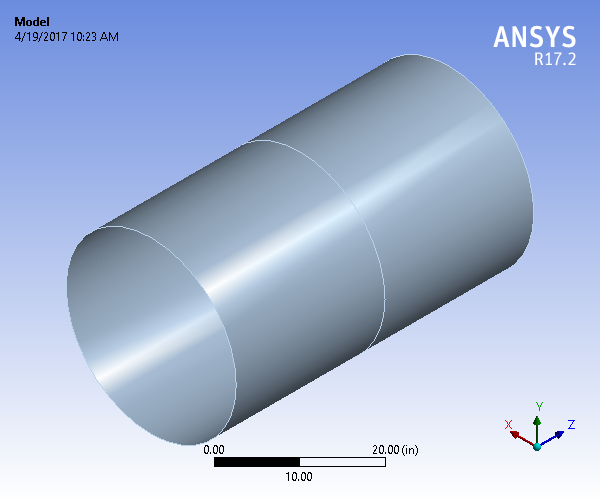
\includegraphics[scale=0.5]{4_geom}
	\caption{Geometry and coordinate system overview.}
	\label{fig:4_geom}
\end{figure}

In this model, the drum's thin surface has a parameterized inward thickness. Parametric studies will be performed in ANSYS with this variable to see how maximum stress and deformation vary. The thin surface also allows for a simply initial coarse mesh generated in ANSYS (see Figure~\ref{fig:4_mesh}).

\begin{figure}[H]
	\centering
	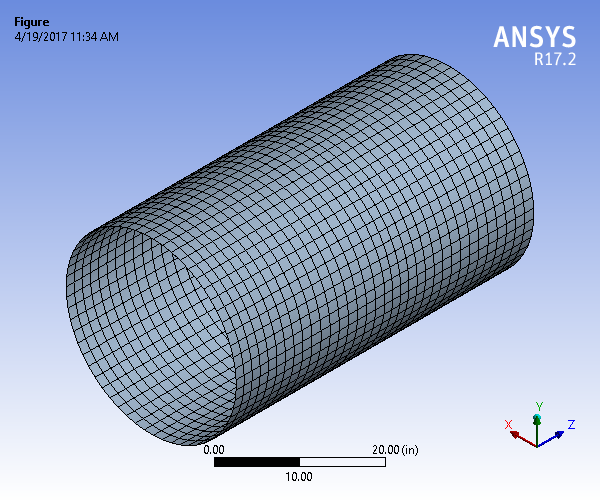
\includegraphics[scale=0.5]{4_mesh}
	\caption{ANSYS generated coarse mesh.}
	\label{fig:4_mesh}
\end{figure}

To assure numerically accurate results, a mesh refinement study will be performed on both maximum total deformation and equivalent (Von-Misses) stress for all foregoing simulations.



\section{Run 1: Uniform Pressure}

The initial FEA run will have a simplistic case. 

\subsection{Boundary Conditions}
\label{subsection:R1BC}
Both of the drum's ends are fixed (i.e. BCs as per \ref{eq:2_fixedBC}).\\

Figure~\ref{fig:4_R1_p} shows uniform external pressure of $1376 \Unit{psi}$ or $9.484 \Unit{MPa}$ as per \ref{eq:2_preq}.
\begin{figure}[H]
	\centering
	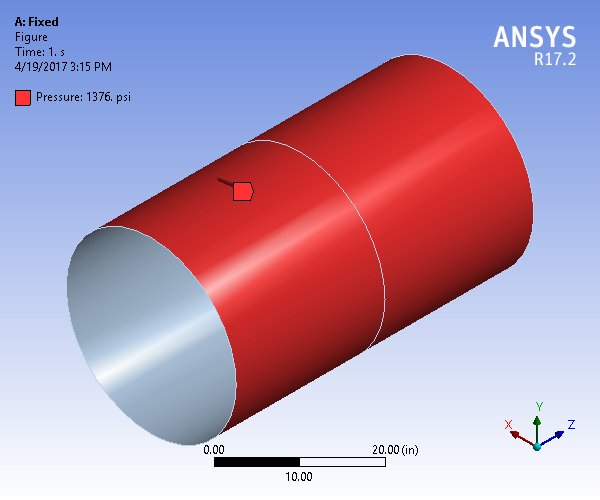
\includegraphics[scale=0.5]{4_R1_p}
	\caption{Uniform external pressure on model.}
	\label{fig:4_R1_p}
\end{figure}

\subsection{Results}

After a mesh refinement, total deformation results are shown below in Figure~\ref{fig:4_R1_def}. The maximum deformation seen on the top surface of the drum in the $y$ direction with respect to $z$ are also shown in Figure~\ref{fig:4_R1_topdef}. Note results shown for $t=0.50\Unit{in}$

\begin{figure}[H]
	\centering
	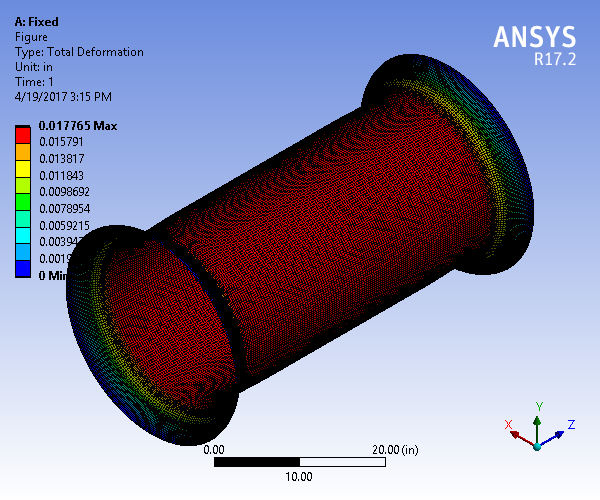
\includegraphics[scale=0.5]{4_R1_def}
	\caption{Total deformation results.}
	\label{fig:4_R1_def}
\end{figure}
\begin{figure}[H]
	\centering
	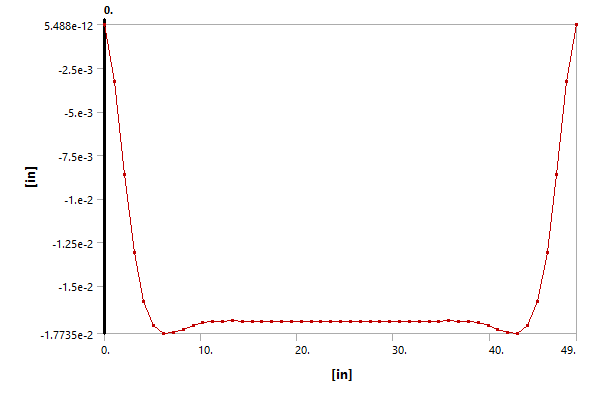
\includegraphics[scale=0.6]{4_R1_topdef}
	\caption{Total deformation in $y$ as a function of $z$.}
	\label{fig:4_R1_topdef}
\end{figure}

Comments, lots of deformation.\\

Again, post mesh refinement yields the maximum stress results as per Figure~\ref{fig:4_R1_stress}.

\begin{figure}[H]
	\centering
	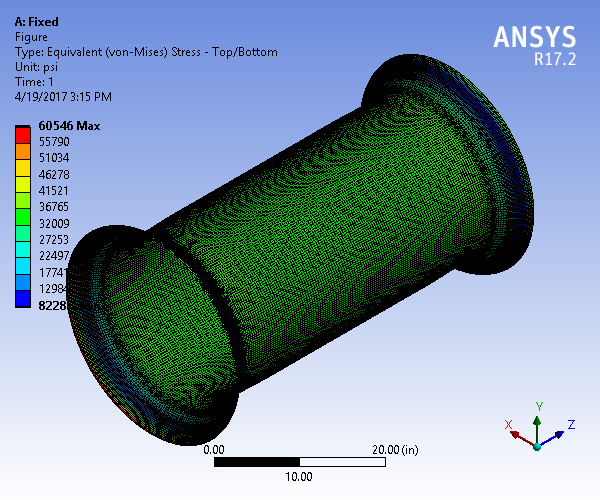
\includegraphics[scale=0.5]{4_R1_stress}
	\caption{Total stress results.}
	\label{fig:4_R1_stress}
\end{figure}

Comments, bad stress.


\subsection{Parametric Study}

A parametric study was ran with $t \in [0.50, 1.75]$. This sweep results are shown below in Figure~\ref{fig:4_R1_sweep} \cite{EXCEL}. The allowable stress limit of Equation~\ref{eq:2_sigall} of $23,333 \Unit{psi}$ is also shown for reference.

\begin{figure}[H]
	\centering
	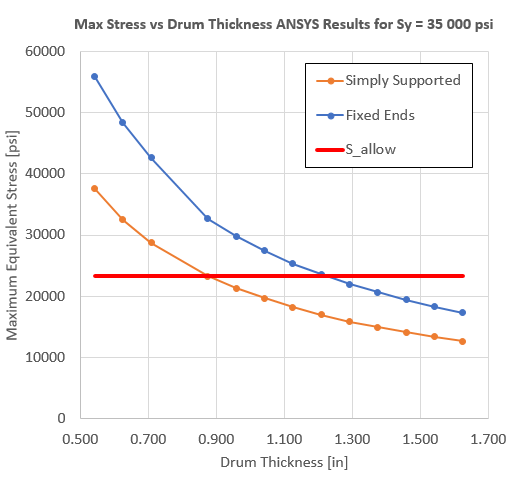
\includegraphics[]{4_R1_sweep}
	\caption{Results of parametric study for FEA Run 1.}
	\label{fig:4_R1_sweep}
\end{figure}

From the above plot, it appears as though a thickness of $t \approx 1.25 \ in$ would appear to be sufficient.

\section{Run 2: Capstan Pressure}

The second run continues on the results determined from Run 1. The results presented in this foregoing section will focus on a barrel thickness of $0.50\ in$.

\subsection{Boundary Conditions}

Both of the drum's ends are simply supported (i.e. BCs as per \ref{eq:2_endBC} ). In other words, simple supports carry no end moments.\\

Figure~\ref{fig:4_R2_tens} shows the location of applied tether tension of $11,525\ lbs.$ or $51,264\ N$.
\begin{figure}[H]
	\centering
	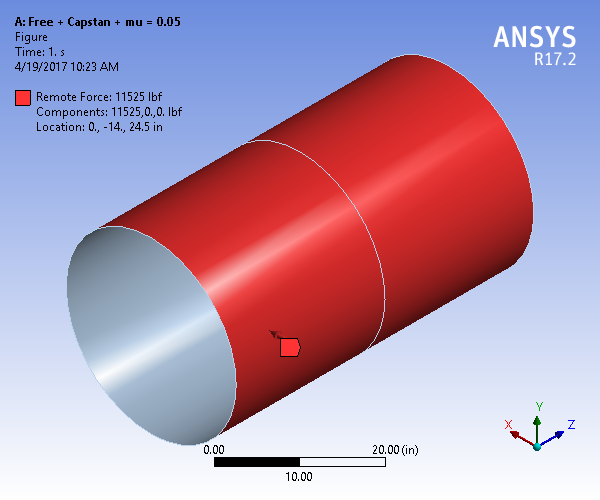
\includegraphics[scale=0.5]{4_R2_tens}
	\caption{Remote force location in ANSYS model.}
	\label{fig:4_R2_tens}
\end{figure}

Figure~\ref{fig:4_R2_pvar} shows the variable Capstan pressure applied as per results from \ref{subsection:alt} (see Figure~\ref{fig:4_R2_pvarplot} for $p(z)$ ). Note again that the boundary conditions are for $\mu=0.05$ , which is essentially the worst case scenario. Note results shown for $t=0.50\ in$

\begin{figure}[H]
	\centering
	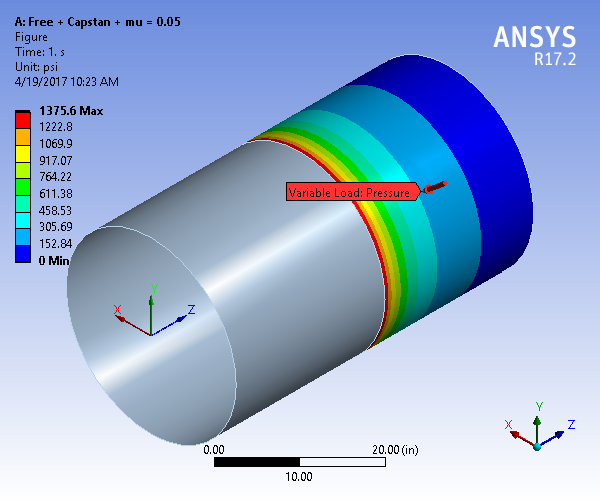
\includegraphics[scale=0.5]{4_R2_pvar}
	\caption{Variable Capstan pressure.}
	\label{fig:4_R2_pvar}
\end{figure}
\begin{figure}[H]
	\centering
	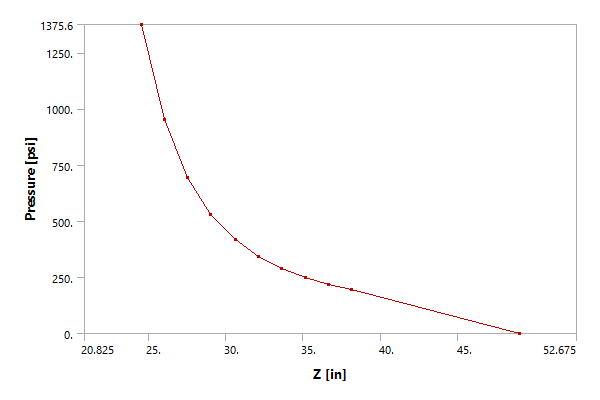
\includegraphics[scale=0.6]{4_R2_pvarplot}
	\caption{Variable Capstan pressure as a function of longitudinal coordinate $z$.}
	\label{fig:4_R2_pvarplot}
\end{figure}


\subsection{Results}

After a mesh refinement, total deformation results are shown below in Figure~\ref{fig:4_R2_def_mu05}. The maximum deformation seen on the top surface of the drum in the $y$ direction with respect to $z$ are also shown in Figure~\ref{fig:4_R2_topdefplotmu05}.

\begin{figure}[H]
	\centering
	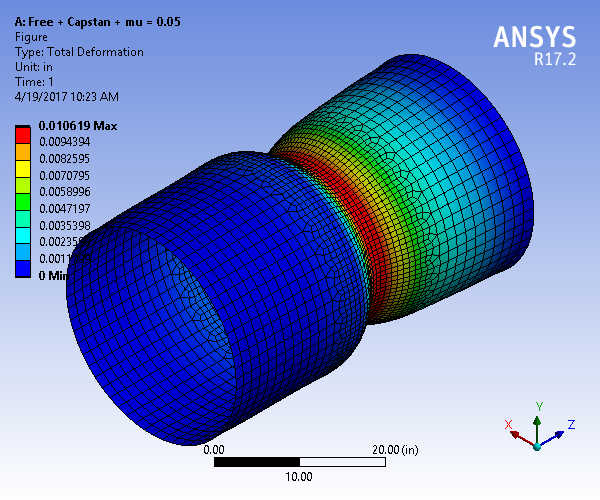
\includegraphics[scale=0.5]{4_R2_def_mu05}
	\caption{Total deformation results.}
	\label{fig:4_R2_def_mu05}
\end{figure}
\begin{figure}[H]
	\centering
	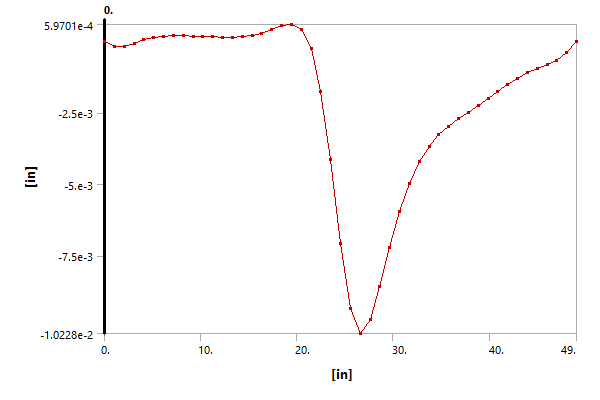
\includegraphics[scale=0.6]{4_R2_topdefplotmu05}
	\caption{Total deformation in $y$ as a function of $z$.}
	\label{fig:4_R2_topdefplotmu05}
\end{figure}

Comments, lots of deformation.\\

Again, post mesh refinement yields the maximum stress results as per Figure~\ref{fig:4_R2_stress_mu05}.

\begin{figure}[H]
	\centering
	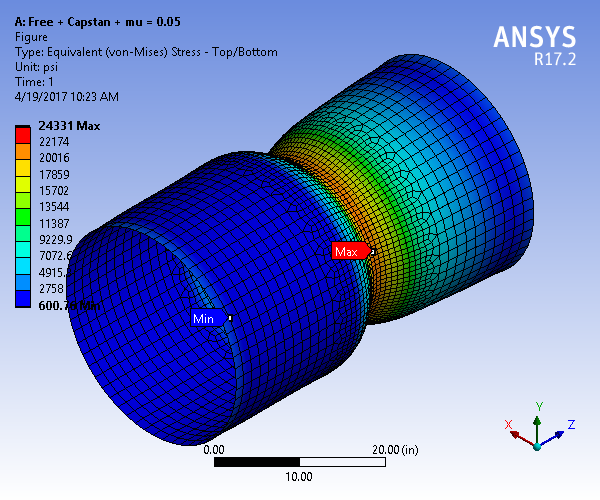
\includegraphics[scale=0.5]{4_R2_stress_mu05}
	\caption{Total stress results.}
	\label{fig:4_R2_stress_mu05}
\end{figure}

Comments, bad stress.


\subsection{Parametric Study}

A parametric study was ran with $0.15 \leq t \leq 1.05$ and $0.05 \leq \mu \leq 0.50$. This sweep results are shown below in Figure~\ref{fig:4_R2_sweep} \cite{EXCEL}.  The allowable stress limit of Equation~\ref{eq:2_sigall} of $23,333 \Unit{psi}$ is also shown for reference.

\begin{figure}[H]
	\centering
	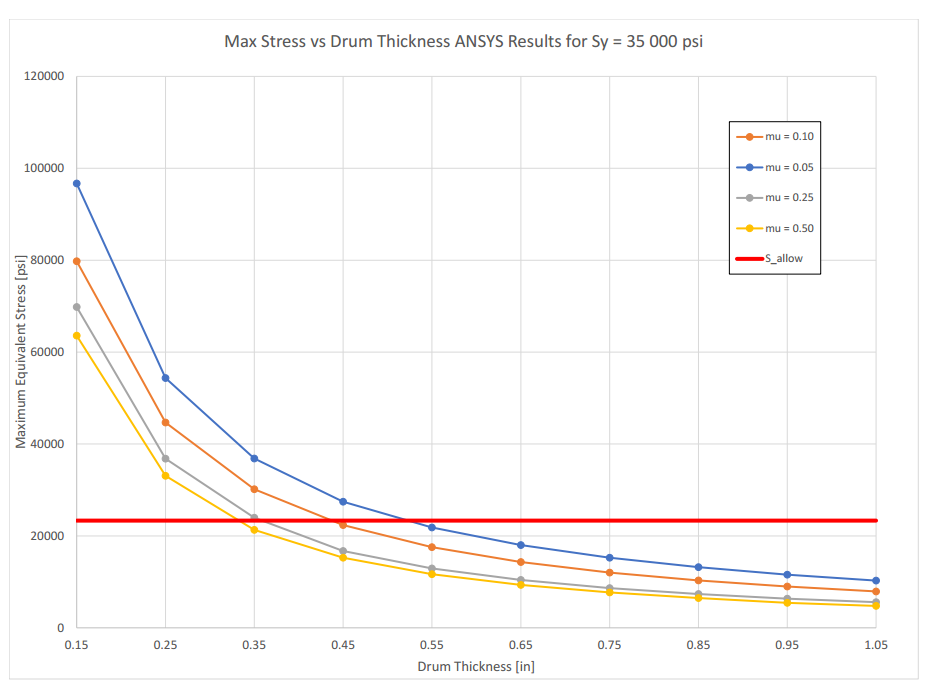
\includegraphics[]{4_R2_sweep}
	\caption{Results of parametric study for FEA Run 2.}
	\label{fig:4_R2_sweep}
\end{figure}

From the above plot, it appears as though a thickness of $t \geq 0.50\ in$ would appear to be sufficient.


\section{Run 3: Eigenvalue Buckling}

Very unconservative \\

Buckling mode shapes do not represent actual displacements but help you to visualize how a part or an assembly deforms when buckling. \cite{ANSYS}. \\

Load factors $\lambda$ highly dependent on pre-stressed state, either linear on non linear.\\

In this case linear buckling is utilized for its simplicity. Must have coupled static structural analysis (see Figure~\ref{fig:4_R3_wb}.

\begin{figure}[H]
	\centering
	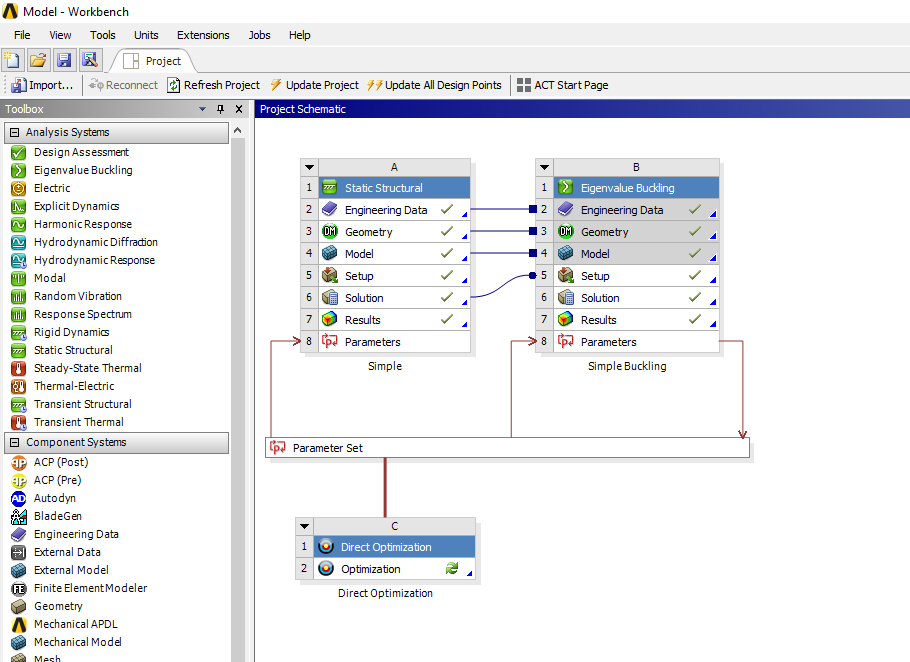
\includegraphics[scale=0.5]{4_R3_wb}
	\caption{Workbench project schematic.}
	\label{fig:4_R3_wb}
\end{figure}

ANSYS takes in the pre-stressed state and returns load factors $\lambda$ which are defined as follows in Equation~\ref{eq:4_loadfactor}.
\begin{equation}
	\label{eq:4_loadfactor}
	p' = \lambda \ p_0
\end{equation}

For this reason, a unit load pressure of $p_0 = 1\ psi$ will be applied. The boundary conditions will follow those of Section~\ref{subsection:R1BC}.

\subsection{Boundary Conditions}

Boundary conditions of coupled static structural analysis. Ends simply supported (Equation~\ref{eq:2_endBC}) and a unit pressure load applied to external surface (see Figure~\ref{fig:4_R3_BC}). Furthermore, for comparison of critical buckling calculations in Section~\ref{section:3_buckle}, a thickness of $t=0.418\ in$ was modeled. 

\begin{figure}[H]
	\centering
	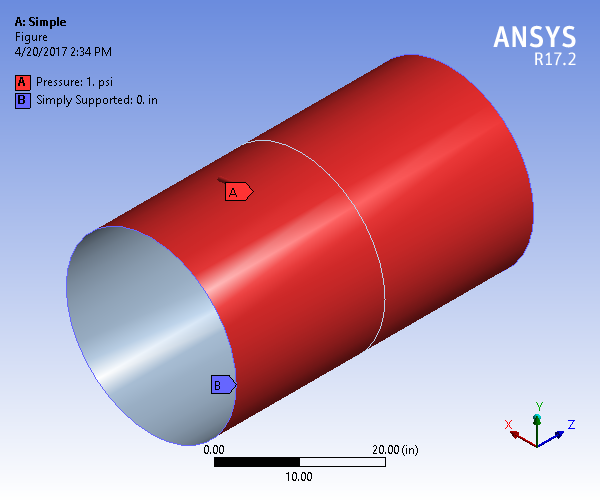
\includegraphics[scale=0.5]{4_R3_BC}
	\caption{Boundary conditions for Eigenvalue Buckling analysis.}
	\label{fig:4_R3_BC}
\end{figure}

\subsection{Results}

Unfortunately, ANSYS is unable to perform a mesh refinement study for a coupled static structural and eigenvalue buckling analysis hence, a much finer initial mesh than that shown in Figure~\ref{fig:4_mesh} was used to assure reasonably accurate results on the first iteration.\\

Results are shown below for the first eigenvalue or mode $\psi = 1$ below in Figure~\ref{fig:4_R3_mode1}.
\begin{figure}[H]
	\centering
	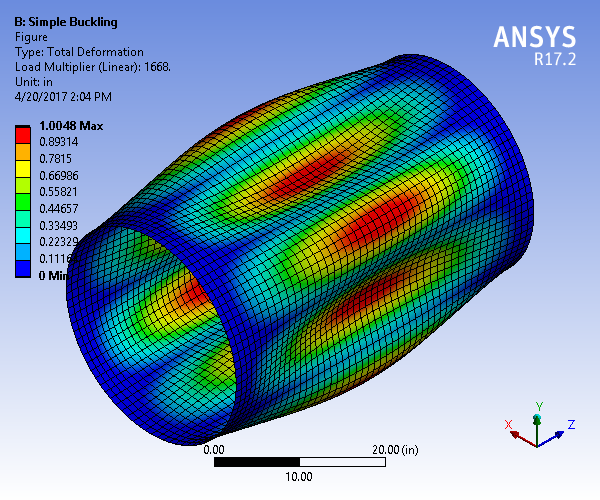
\includegraphics[scale=0.5]{4_R3_mode1}
	\caption{Total deformation results for mode $\psi = 1$.}
	\label{fig:4_R3_mode1}
\end{figure}

From above, it can be seen that a load factor of $\lambda = 1668$ was calculated for $t= 0.418\Unit in$. This value is within about $21.2\%$ of the expected analytical results.

\subsection{Parametric Study}

For $t\in [0.05, 1.05]$, a parametric study was performed. Results for the first, fifth and tenth mode (i.e. $\psi = 1, 5, 10$) are plotted against the thickness range of interest in Figure~\ref{fig:4_R3_modesweep} below, as per \cite{PYTHON} script in Appendix~\ref{appendix:a4}. The required critical pressure of $p =1376\ psi$ is also shown for reference.

\begin{figure}[H]
	\centering
	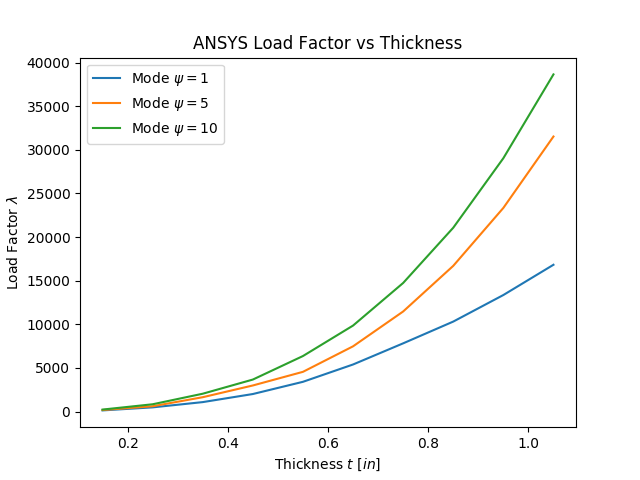
\includegraphics[scale=0.75]{4_R3_modesweep}
	\caption{Parametric sweep results for various $t, \psi$.}
	\label{fig:4_R3_modesweep}
\end{figure}

\begin{figure}[H]
	\centering
	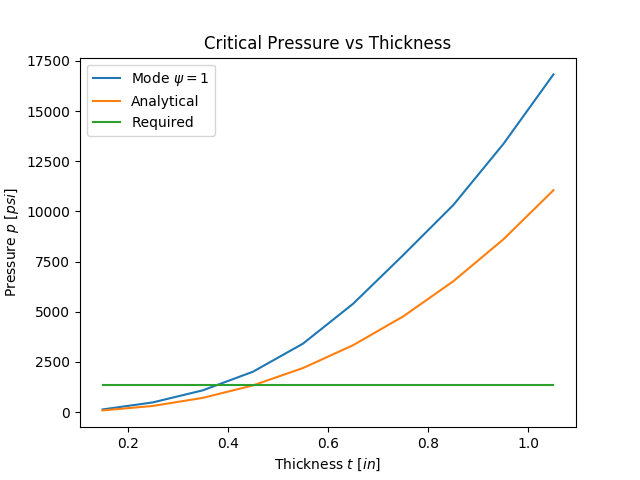
\includegraphics[scale=0.75]{4_R3_comp}
	\caption{Comparison of analytical and FEA results.}
	\label{fig:4_R3_comp}
\end{figure}


